%% To submit your paper:
%DIF LATEXDIFF DIFFERENCE FILE
%DIF DEL paper.tex     Thu Dec 29 16:43:33 2016
%DIF ADD paperMD.tex   Thu Dec 29 16:53:00 2016
\documentclass[draft,linenumbers]{agujournal}
\draftfalse

%% For final version.
% \documentclass{agujournal}

\journalname{Water Resources Research}

\usepackage{url, bbm, comment}
%DIF PREAMBLE EXTENSION ADDED BY LATEXDIFF
%DIF UNDERLINE PREAMBLE %DIF PREAMBLE
\RequirePackage[normalem]{ulem} %DIF PREAMBLE
\RequirePackage{color}\definecolor{RED}{rgb}{1,0,0}\definecolor{BLUE}{rgb}{0,0,1} %DIF PREAMBLE
\providecommand{\DIFadd}[1]{{\protect\color{blue}\uwave{#1}}} %DIF PREAMBLE
\providecommand{\DIFdel}[1]{{\protect\color{red}\sout{#1}}}                      %DIF PREAMBLE
%DIF SAFE PREAMBLE %DIF PREAMBLE
\providecommand{\DIFaddbegin}{} %DIF PREAMBLE
\providecommand{\DIFaddend}{} %DIF PREAMBLE
\providecommand{\DIFdelbegin}{} %DIF PREAMBLE
\providecommand{\DIFdelend}{} %DIF PREAMBLE
%DIF FLOATSAFE PREAMBLE %DIF PREAMBLE
\providecommand{\DIFaddFL}[1]{\DIFadd{#1}} %DIF PREAMBLE
\providecommand{\DIFdelFL}[1]{\DIFdel{#1}} %DIF PREAMBLE
\providecommand{\DIFaddbeginFL}{} %DIF PREAMBLE
\providecommand{\DIFaddendFL}{} %DIF PREAMBLE
\providecommand{\DIFdelbeginFL}{} %DIF PREAMBLE
\providecommand{\DIFdelendFL}{} %DIF PREAMBLE
%DIF END PREAMBLE EXTENSION ADDED BY LATEXDIFF

\begin{document}


\title{I don't know, are you sure we want to do this?\\
Sea level adaptation decisions under uncertainty}

\DIFdelbegin %DIFDELCMD < \authors{T. L. Thorarinsdottir\affil{1}, P. Guttorp\affil{1}, M. Drews\affil{2}, and K. de Bruin\affil{3,4}}
%DIFDELCMD < %%%
\DIFdelend \DIFaddbegin \authors{T. L. Thorarinsdottir\affil{1}, P. Guttorp\affil{1}, M. Drews\affil{2}, K. de Bruin\affil{3,4}, and P. S. Kaspersen\affil{2}}
\DIFaddend 

\affiliation{1}{Norwegian Computing Center, Oslo, Norway}
\DIFdelbegin %DIFDELCMD < \affiliation{2}{Technical University of Denmark, Copenhagen, Denmark}
%DIFDELCMD < %%%
\DIFdelend \DIFaddbegin \affiliation{2}{Technical University of Denmark, Kgs. Lyngby, Denmark}
\DIFaddend \affiliation{3}{Center for International Climate and Environmental Research, Oslo, Norway}
\affiliation{4}{Wageningen Environmental Research, Wageningen, The Netherlands}

\correspondingauthor{T. L. Thorarinsdottir}{thordis@nr.no}

\begin{keypoints}
\item Decisions on adaptation measures need to take careful account of \DIFdelbegin \DIFdel{uncertainties
}\DIFdelend \DIFaddbegin \DIFadd{uncertanties
}\DIFaddend \item More careful models are needed for increased costs of the effects of sea level rise
\item \DIFdelbegin \DIFdel{Modeling }\DIFdelend \DIFaddbegin \DIFadd{Modelling }\DIFaddend local sea level rise is essential
\end{keypoints}


\begin{abstract}
Sea level rise has serious consequences for harbor infrastructure, storm drains and sewer systems, and many other issues. Adapting to sea level rise requires comparing different possible adaptation strategies, comparing the cost of different actions (including no action), and assessing at what point in time the chosen strategy should be implemented. All these decisions must be made under considerable uncertainty--in the amount of sea level rise, in the cost of adaptation actions, \DIFdelbegin \DIFdel{and }\DIFdelend in the cost of no action. We develop two illustrative examples: for Bergen on Norway's west coast and for Esbjerg on the west coast of Denmark. Different components of uncertainty are visualized. \DIFdelbegin \DIFdel{We show that failing to take uncertainty into account can increase the projected damage costs by an order of magnitude.
}\DIFdelend \DIFaddbegin {\color{blue} \DIFadd{Findings go here}}
\DIFaddend \end{abstract}


%% ------------------------------------------------------------------------ %%
%  BEGIN ARTICLE
%% ------------------------------------------------------------------------ %%


\section{Introduction}\label{sec:intro}
\DIFdelbegin \DIFdel{Long-term planning and decision-making regarding societal infrastructure along coastal areas must account for a changing climate. In particular, potential changes in }\DIFdelend \DIFaddbegin \DIFadd{The potential impact of climate change on }\DIFaddend local sea level\DIFdelbegin \DIFdel{can yield numerous }\DIFdelend \DIFaddbegin \DIFadd{, yielding }\DIFaddend effects such as frequent flooding, inundation and \DIFdelbegin \DIFdel{back flow }\DIFdelend \DIFaddbegin \DIFadd{backflow }\DIFaddend of storm drainage and sewer systems, destructive erosion and contamination of wetlands and other habitats\DIFdelbegin \DIFdel{. Considerable challenges continue to exist in understanding  the impacts of a combination of sea level rise and storm surges and the implementation of potential adaptation options to reduce these impacts. Severe inherent uncertainties persist along all parts of the processing chain from climate projections to adaptation assessments, and it is critical that decision-making appropriately accounts for this.
 }%DIFDELCMD < 

%DIFDELCMD < %%%
\DIFdel{As adaptation decision-making is an ongoing process of weighing and choosing which measures should be taken at which moment in time \mbox{%DIFAUXCMD
\citep{Hallegatte&2012} }%DIFAUXCMD
adaptive planning methods need to support }\DIFdelend \DIFaddbegin \DIFadd{, requires city planners to make }\DIFaddend decisions in the \DIFdelbegin \DIFdel{short term, while considering long-term developments. Challenges of adaptation decision-making under uncertaintyrelate to the incorporation of spatial, inter-temporal and flexibility aspects of adaptation priorities \mbox{%DIFAUXCMD
\citep{FankhauserSoare2013}}%DIFAUXCMD
, and the linkage with specific characteristics of sectors and contexts \mbox{%DIFAUXCMD
\citep{BisaroSwartHinkel2016, HinkelBisaro2016}}%DIFAUXCMD
. Several economic decision support tools and methods exist for adaptation assessment under uncertainty \mbox{%DIFAUXCMD
\citep[e.g.][]{Chambwera&2014, WilbyDessai2010, WalkerHaasnootKwakkel2013}}%DIFAUXCMD
. However, \mbox{%DIFAUXCMD
\citet{Watkiss&2015} }%DIFAUXCMD
conclude that these tools are very resource intensive and complex }\DIFdelend \DIFaddbegin \DIFadd{presence of substantial uncertainty.
}

\DIFadd{In this paper we demonstrate the importance of combining projections of sea level rise and flood damages alongside a detailed quantification of both hydrologic and economic uncertainties }\DIFaddend in the context of \DIFdelbegin \DIFdel{long-term adaptation investment decisions and call for the development of ``light touch'' approaches to better support local adaptation making. }%DIFDELCMD < 

%DIFDELCMD < %%%
\DIFdel{In this paper we combine the uncertainty of sea level projections with a simplified decision framework under uncertainty where }\DIFdelend \DIFaddbegin \DIFadd{real-life decision-problems experienced by stakeholders and authorities in Bergen and Esbjerg. Based on communications with local end-users we highlight the value of taking into account uncertainty through two simplified and complementary case studies, where in the first one  }\DIFaddend planners want to know how early they should implement costly adaptation measures\DIFdelbegin \DIFdel{.  We discuss the advantages of using a fully probabilistic approach in a light touch decision framework that accounts for uncertainty both in climate projections and damage assessments, where information on uncertainty is turned into a driver of change rather than a barrier. }\DIFdelend \DIFaddbegin \DIFadd{, whereas in the second case the aim is to highlight the risk of flooding in coastal areas, e.g. in order to prioritize future adaptation actions and investments. In both cases we show that embracing the uncertainties derived from economic and hydrologic models is absolutely crucial in order to answer the question of "are we sure we want to do this?". 
}\DIFaddend 

\DIFdelbegin %DIFDELCMD < \begin{figure}[!hbpt]
%DIFDELCMD < \begin{center}
%DIFDELCMD <   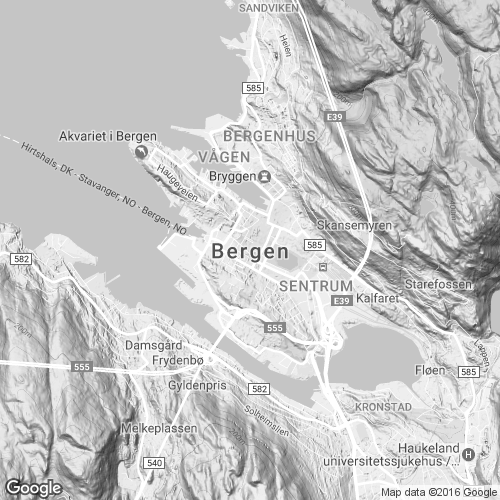
\includegraphics[width=0.45\linewidth]{BergenMap.png}
%DIFDELCMD <   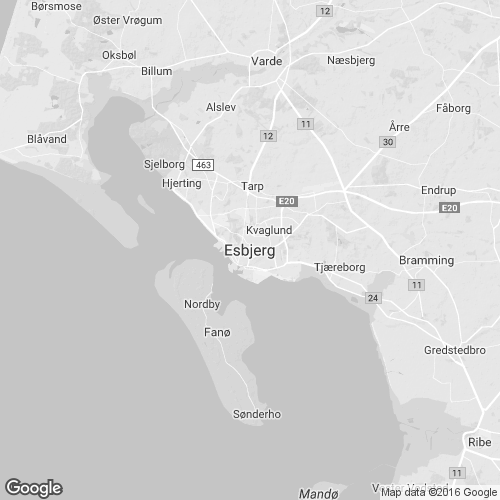
\includegraphics[width=0.45\linewidth]{EsbjergMap.png}
%DIFDELCMD < %%%
%DIFDELCMD < \caption{%
{%DIFAUXCMD
\DIFdelFL{Terrain maps of central Bergen, Norway (left) and Esbjerg, Denmark (right).}}
%DIFAUXCMD
%DIFDELCMD < %DIFDELCMD < \label{fig:CityMaps}%%%
%DIFDELCMD < \end{center}
%DIFDELCMD < \end{figure}
%DIFDELCMD < 

%DIFDELCMD < %%%
\DIFdel{We illustrate the sea level rise projections and timing of adaptation measures for two case studies in Northern Europe, namely the city of Bergen in Norway and Esbjerg in Denmark, see Figure~\ref{fig:CityMaps}. 
}\DIFdelend The Norwegian city of Bergen is the capital of Hordaland County. The city center is located on Byfjorden, and is surrounded by mountains. It has the largest port in Norway, both in terms of freight and passengers. The historic harbor area, Bryggen, is the only Hanseatic trade center remaining in its original style, and has been declared a \DIFdelbegin \DIFdel{UN-ESCO }\DIFdelend \DIFaddbegin \DIFadd{UNESCO }\DIFaddend World Heritage site \DIFdelbegin \footnote{\DIFdel{See }%DIFDELCMD < \url{http://whc.unesco.org/en/list/59}%%%
\DIFdel{.}}%DIFAUXCMD
\addtocounter{footnote}{-1}%DIFAUXCMD
\DIFdelend \DIFaddbegin \DIFadd{(}\url{http://whc.unesco.org/en/list/59}\DIFadd{)}\DIFaddend . Bryggen is regularly flooded at extreme tides, and it is feared that as sea levels rise, floods will become a major problem in other parts of Bergen as well \citep{bergenreport}.

\DIFdelbegin \DIFdel{The municipality of Bergen has, }\DIFdelend \DIFaddbegin \DIFadd{Esbjerg, on the southwest coast of Jutland, is the fifth-largest city in Denmark and the largest urban area }\DIFaddend in \DIFdelbegin \DIFdel{cooperation with private actors, analyzed several possible adaptation measures against sea level rise. The measures range from an outer barrier that would protect the entire metropolitan area to various protection measures of limited areas in the inner harbor \mbox{%DIFAUXCMD
\citep{bergenreport}}%DIFAUXCMD
. While the viability of the constructions and the associated construction costs have been carefully analyzed, }\DIFdelend the \DIFdelbegin \DIFdel{optimal timing of potential adaptation measures and the effects of the associated uncertainties have yet to be investigated. We perform such an analysis where we consider uncertainty in projected sea level rise, damage costs and the effects of sea level rise on changes in damage costs.  }%DIFDELCMD < 

%DIFDELCMD < %%%
\DIFdel{Esbjerg , on the west coast of Jutland, has the second largest harbor in Denmark. It can be subjected to substantial storm surges, which , in conjunction with heavy rainfall, can flood substantial parts of the town.
 }\DIFdelend \DIFaddbegin \DIFadd{region. The city hosts one of the largest harbours  in Denmark, which serves as a focal point for offshore activities in the North Sea, including the continued development of offshore wind power and extensive activities related to the extraction of oil and gas. As a result critical infrastructures and commercial buildings figure prominently in the coastal zone. Esbjerg is frequently subject to substantial storms and storm surges, causing severe flooding of the harbour and the city. The highest ever since 1874 was recorded in 1981, where the harbour was completely flooded and the water level reached a record-high 433 cm above the norm, causing massive economic losses.  More generally, storm surges causing water levels in Esbjerg to rise to between 2 and 3 metres have quadrupled over the last four decades according to local records, whereas half of the most severe events have taken place since 1975. As in the case of Bergen, sea level rise caused by climate change is expected to compound these risks, alongside parallel threats caused by increased risks of pluvial flooding and rising ground water levels in Esbjerg. The municipality recently adopted its climate adaptation plan, which in its first phase is aimed at identifying present and future flood-prone areas, e.g. to avoid urban development into such areas, to limit damages to buildings of high societal or cultural value, and to pave the way for implementing cost-effective adaptation measures in the second phase of the plan.   
 }\DIFaddend 

\DIFdelbegin \DIFdel{The remainder of the paper is organized as follows.   
 }\DIFdelend Section \ref{sealevelproj} describes our approach to projecting sea level. In section \DIFdelbegin \DIFdel{\ref{decision_tools_PartI} }\DIFdelend \DIFaddbegin \DIFadd{\ref{decision_tools} }\DIFaddend we describe the \DIFdelbegin \DIFdel{decision framework focused on the timing of proactive adaptation decision }\DIFdelend \DIFaddbegin \DIFadd{type of decision problem that we are going to attack}\DIFaddend . We apply \DIFdelbegin \DIFdel{this framework }\DIFdelend \DIFaddbegin \DIFadd{these tools }\DIFaddend to  sea level projections \DIFdelbegin \DIFdel{and adaptation }\DIFdelend for Bergen, Norway, and for Esbjerg, Denmark 
in section \ref{cases}.  In the final section \ref{unc}  we demonstrate the consequences of ignoring the uncertainty in the projections.

\section{Sea level projections \DIFaddbegin {\color{blue} \DIFadd{(PG)}}\DIFaddend }
\DIFaddbegin 

\DIFaddend \label{sealevelproj}

\DIFdelbegin \DIFdel{We project local sea level changes by Modeling two processes, the relationship between global temperature and global sea level, and the relationship between global sea level and local sea level.
}%DIFDELCMD < 

%DIFDELCMD < %%%
\DIFdelend \subsection{Global sea level}
Most climate models do not explicitly provide sea level as an output of the calculations. Rather, the IPCC AR5 report \citep[ch.~13]{ipcc} combines the heat expansion of the ocean with temperature forced models for glacial melt, Greenland ice melt, and Antarctic ice melt and with land rise due to rebound from the last ice age. Judging from the supplementary material to \citet[ch.~13]{ipcc}, the uncertainty assessment is only based on the spread of the ensemble of temperature projections, not on the additional uncertainty in the ice models used.

We will instead use the empirical approach of Rahmstorf and collaborators \citep{Rahmstorf07,Rahmstorf11}, employing the statistical modeling of \citet{Bolin2014a} to relate global annual mean temperature anomalies to global mean sea level anomalies. 


We then apply the estimated historical relationship to projected temperatures from the CMIP5 experiment \citep{cmip5} to obtain projected global annual mean sea level, taking into account the uncertainty in the statistical model as well as the spread of the temperature projection ensemble (see subsection \ref{unc_ass}). 
For the i'th temperature projection $T_t^i$ we estimate the corresponding global mean sea level as
\DIFdelbegin %DIFDELCMD < \begin{linenomath*}
%DIFDELCMD < %%%
\DIFdelend \DIFaddbegin 

\DIFaddend \[H_t^{gl,i} = \int\limits_{{t_0}}^t {{\hat a} (T_u^i - {{\hat T}_0}} )du + {\varsigma _t}\DIFdelbegin \DIFdel{,}\DIFdelend \]
\DIFdelbegin %DIFDELCMD < \end{linenomath*}
%DIFDELCMD < %%%
\DIFdelend where ${\hat a}$ and ${\hat T}_0$ are regression parameters of observed global sea level  rise on observed global temperature and $\varsigma_t$ the integrated time series regression error.



\subsection{Local sea level}
In order to get from global sea level projections to local ones, it is important to note that sea level rise \DIFdelbegin \DIFdel{is not }\DIFdelend \DIFaddbegin \DIFadd{not is }\DIFaddend uniform over the globe. Glacial and land ice melting affect the local sea level differently depending on where the melted ice is located.
%Gravitational effects
Another major effect in Fennoskandia is the land rise due to isostatic rebound from the glaciers of the last ice age. 
Again, we will use historical data to relate global sea level to isostatically corrected local sea level using a time series regression model. 
The local sea level projections are then obtained by first relating projected temperature to global sea level, and then relating the global sea level to the local one. Each climate model temperature projection yields a different local sea level projection. The local sea level projection based on the i'th climate model for years beyond 2000 is estimated as
\DIFdelbegin %DIFDELCMD < \begin{linenomath*}
%DIFDELCMD < %%%
\DIFdelend \DIFaddbegin 

\DIFaddend \[H_t^{loc,i} + \gamma (t -2000 ) = {\hat b} H_t^{gl,i}  + {\varepsilon _t}\DIFdelbegin \DIFdel{,}\DIFdelend \]
\DIFdelbegin %DIFDELCMD < \end{linenomath*}
%DIFDELCMD < %%%
\DIFdelend \DIFaddbegin 


\DIFaddend where $\gamma$ is the annual land rise rate, $t$ denotes year, and $ {\hat b} $ is the regression coefficient relating global to local sea level.




\subsection{Uncertainty assessment}
\label{unc_ass}
Following the approach of \citet{Guttorp2014} we assess the uncertainty in the local sea level projections taking into account the variability between the climate projections used, the uncertainties in the regressions of global mean temperature on global mean sea level and of global on local sea level. We express the sea level projection uncertainty in terms of a confidence band that is simultaneously of the intended  level  for all projection years. This allows us, for example, to get a confidence band for the years when a given sea level rise is obtained. 



\subsection{Limitations of the sea level projections}
The main assumption is using historical relationships in statistical projections of the type used in this paper is that there is no major change in how temperature relates to sea level, globally and locally. Among the factors that may invalidate this approach are changes in water storage on land (in essence removing water from the oceans), excessive siphoning of groundwater (resulting in land subsidence), changes in the rates of glacial and land ice melt, and changes in Earth's gravitational field due to transfer of mass from land ice to ocean water. For example, the rate of ice melt on Greenland may suddenly increase substantially due to intense warming of both air and sea water \citep{bamber2013}. A recent paper \citep{jevrejeva2016} indicates that the upper tails of sea level rise may be substantially higher when taking into account expert assessment of land ice melting. Our current climate models are not able to resolve the ice processes sufficiently to include such so called tipping points into the projections. Also, the IPCC scenarios \citep{change} do not include changes in water usage (cf. \citet{wada2012}). 

\section{\DIFdelbegin \DIFdel{Timing of adaptation measures}\DIFdelend \DIFaddbegin \DIFadd{Decision tools }{\color{blue} \DIFadd{(KdB, MD, TT)}}\DIFaddend }
\DIFdelbegin %DIFDELCMD < \label{decision_tools_PartI}
%DIFDELCMD < %%%
\DIFdelend \DIFaddbegin \label{decision_tools}
\DIFaddend 

\DIFdelbegin \DIFdel{To assess the optimal timing of an adaptation measure, we employ a probabilistic extension of the framework described by \mbox{%DIFAUXCMD
\citep{Fankhauser&1999} }%DIFAUXCMD
in which we obtain a probabilistic distribution for the net present value damage in a given year for various adaptation options. The probabilistic distribution isconstructed by considering uncertainty in the local sea level projections, in the annual damage costs, and in the effect of changes in sea level on the annual damage costs. }\DIFdelend \DIFaddbegin \subsection{\DIFadd{Timing of adaptation measures}}
\DIFaddend 

\DIFdelbegin \subsection{\DIFdel{Annual damage costs}} 
%DIFAUXCMD
\addtocounter{subsection}{-1}%DIFAUXCMD
\DIFdelend \DIFaddbegin \DIFadd{We consider adaptation decision making related to the timing of proactive adaptation measures. That is, the goal is to adapt to sea level rise before major damages occur. In a cost-benefit framework, an investment should be delayed as long as the benefits of delay (avoided investment costs) are greater than the associated costs (higher climate change damages) \mbox{%DIFAUXCMD
\citep{Fankhauser&1999}}%DIFAUXCMD
.
}\DIFaddend 

\DIFdelbegin \DIFdel{We }\DIFdelend \DIFaddbegin \DIFadd{We assume that damages related to sea level rise coincide with damages due to storm surges and that the accumulated annual damages are independent between years. More specifically, we }\DIFaddend model the distribution of annual damage, \DIFdelbegin \DIFdel{$F_{\textup{d}, t_0}$, for the year $t_0 = 2015$ }\DIFdelend \DIFaddbegin \DIFadd{$F_{\textup{d}}$, }\DIFaddend by the three parameter Burr distribution \citep{Burr1942} with density
\begin{linenomath*}
  \begin{equation}\label{eq:Burr}
  f\DIFdelbegin \DIFdel{_{\textup{d}, t_0} }\DIFdelend \DIFaddbegin \DIFadd{_{\textup{d}} }\DIFaddend (x) = \frac{\alpha \gamma (x/ \theta)^{\gamma}}{x [ 1 + (x/ \theta)^{\gamma}]^{\alpha + 1}}
  \end{equation}
\end{linenomath*}
for $x > 0$, where $\alpha$ and $\gamma$ are shape parameters with $\alpha, \gamma > 0$, and $\theta >0$ is a scale parameter. The Burr distribution has a heavy upper tail and is commonly used to model damage loss, see e.g. \cite{Klugman&2012}.
\DIFdelbegin \DIFdel{The parameters of the distribution are estimated using historical data for annual storm surge damage. Data prior to 2015 are adjusted to the 2015 level using the consumer price index. After adjustment, we assume stationarity over the period and independence between years.
}\DIFdelend 

Under a constant sea level, we can obtain a sample trajectory $\{d_{t_1}, d_{t_2}, \ldots, d_{t_{85}}\}$ of future annual damages for $t_1 = 2016, \ldots, t_{85} = 2100$ by drawing $85$ i.i.d. values from the estimated \DIFdelbegin \DIFdel{distribution }\DIFdelend \DIFaddbegin \DIFadd{damage distribution for $t_0 = 2015$, }\DIFaddend $\hat{F}_{\textup{d}, t_0}$.  By repeating this process $J$ times, we obtain an \DIFdelbegin \DIFdel{empirical }\DIFdelend \DIFaddbegin \DIFadd{empirial }\DIFaddend damage distribution for each future year $t_i$ given by
\begin{linenomath*}
  \[
  \hat{F}_{\textup{d}, t_i} (x) = \frac{1}{J} \sum_{j=1}^J \mathbbm{1}\DIFdelbegin %DIFDELCMD < \Bigg\{ %%%
\DIFdel{\frac{d_{t_i}^{(j)}}{\prod_{l \leq i} (1 + r_{t_l}) } }\DIFdelend \DIFaddbegin \DIFadd{\{d_{t_i}^{(j)} }\DIFaddend \leq x \DIFdelbegin %DIFDELCMD < \Bigg\}
%DIFDELCMD <   %%%
\DIFdelend \DIFaddbegin \DIFadd{\}
  }\DIFaddend \]
\end{linenomath*}
for $i = 1, \ldots, 85$\DIFdelbegin \DIFdel{, where $r_{t_i}$ is the discount rate for year $t_i$. Alternatively}\DIFdelend \DIFaddbegin \DIFadd{. Similarly}\DIFaddend , we obtain an \DIFdelbegin \DIFdel{empirical }\DIFdelend \DIFaddbegin \DIFadd{empirial }\DIFaddend distribution of the total damage over the period $2016-2100$ by considering \DIFdelbegin %DIFDELCMD < \begin{linenomath*}
%DIFDELCMD <   %%%
\[
  \DIFdel{d_{\textup{total}}^{(j)} = \sum_{i=1}^{85} \frac{d_{t_i}^{(j)}}{\prod_{l \leq i} (1 + r_{t_l})}
  }\]
%DIFAUXCMD
%DIFDELCMD < \end{linenomath*}
%DIFDELCMD < %%%
\DIFdel{and similarly for the cumulative damage}\DIFdelend \DIFaddbegin \DIFadd{$d_{\textup{total}}^{(j)} = \sum_{i=1}^{85} d_{t_i}^{(j)}$}\DIFaddend .  

\DIFdelbegin \subsection{\DIFdel{Effect of changes in sea level}}
%DIFAUXCMD
\addtocounter{subsection}{-1}%DIFAUXCMD
%DIFDELCMD < 

%DIFDELCMD < %%%
\DIFdel{We assume that changes in sea level have a multiplicative effect on the annual damage cost. That is, for a sea level anomaly $s_{t_i}$ in year $t_i > 2015$ }\DIFdelend \DIFaddbegin \DIFadd{Now assume we are given a large sample of projections $\{s_{t_1}^{(j)}, \ldots, s_{t_{85}}^{(j)} \}_{j=1}^J$ for annual sea level rise anomalies }\DIFaddend compared to the 2015 \DIFdelbegin \DIFdel{level, the annual damage cost becomes
}%DIFDELCMD < \begin{linenomath*}
%DIFDELCMD <   %%%
\[
  \DIFdel{g(s_{t_i} | \boldsymbol \beta ) d_{t_i},
  }\]
%DIFAUXCMD
%DIFDELCMD < \end{linenomath*}
%DIFDELCMD < %%%
\DIFdel{where $g( \cdot | \boldsymbol \beta )$ is }\DIFdelend \DIFaddbegin \DIFadd{value for the same time period. We model the relationship between the change in damage and change in sea level by }\DIFaddend a monotonic positive function \DIFdelbegin \DIFdel{with parameter vector  }\DIFdelend \DIFaddbegin \DIFadd{$g(s| \boldsymbol \beta )$ with parameters }\DIFaddend $\boldsymbol \beta$\DIFdelbegin \DIFdel{such that }\DIFdelend \DIFaddbegin \DIFadd{, where }\DIFaddend $g(s|\boldsymbol \beta ) > 1$ for $s>0$ and $g(s|\boldsymbol \beta ) < 1$ for $s < 0$. \DIFdelbegin \DIFdel{\mbox{%DIFAUXCMD
\cite{Hallegatte&2013} }%DIFAUXCMD
estimate a similar effect function valid in 2050 for $s \in \{0,20,40\}$ for 136 coastal cities. Here, we use their results for 15 European cites: Amsterdam, Athens, Barcelona, Dublin, Glasgow, Hamburg, Helsinki, Copenhagen, Lisbon, London, Marseilles, Naples, Porto, Rotterdam and Stockholm.  To obtain a city-specific effect function for a large range of sea level anomalies we employ a linear extrapolation as shown in Figure~\ref{fig:EffectFct}. We then obtain a sample of effect functions $\{g(\cdot|\boldsymbol \beta^{(j)})\}_{j=1}^J$ by sampling with replacement from this ensemble of trajectories with all 15 ensemble members considered equally probable. 
}%DIFDELCMD < 

%DIFDELCMD < \begin{figure}[!hbpt]
%DIFDELCMD < \begin{center}
%DIFDELCMD < 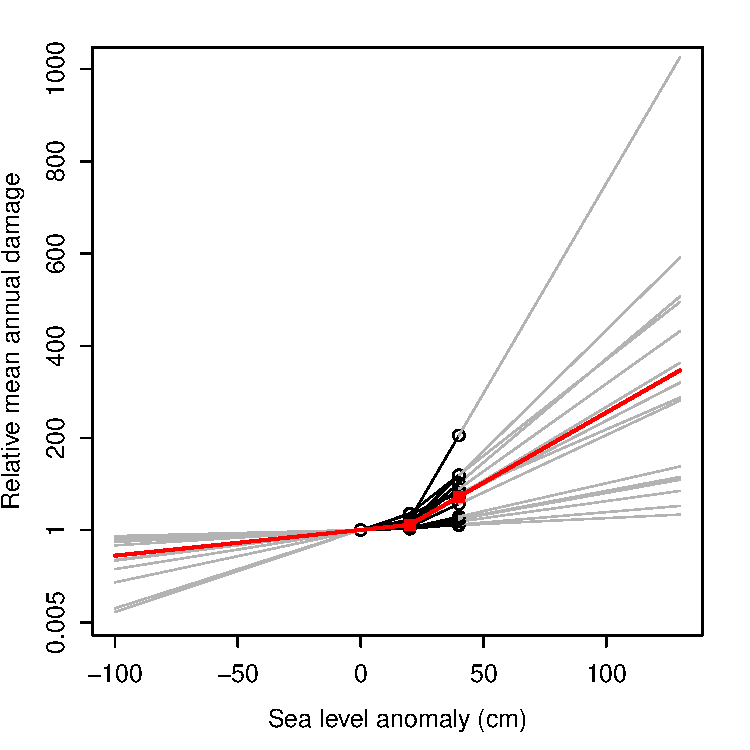
\includegraphics[width=0.5\linewidth]{DecisionAnalysisBergenPartII.pdf}
%DIFDELCMD < %%%
%DIFDELCMD < \caption{%
{%DIFAUXCMD
\DIFdelFL{Relative change in mean annual damage as a function of sea level rise for 15 European cites as estimated by \mbox{%DIFAUXCMD
\cite{Hallegatte&2013} }%DIFAUXCMD
(black circles) with linearly extrapolated values indicated by gray lines. The median change and the corresponding extrapolation are indicated in red.}}
%DIFAUXCMD
%DIFDELCMD < %DIFDELCMD < \label{fig:EffectFct}%%%
%DIFDELCMD < \end{center}
%DIFDELCMD < \end{figure}
%DIFDELCMD < 

%DIFDELCMD < %%%
\DIFdel{Let further $\{s_{t_1}^{(j)}, \ldots, s_{t_{85}}^{(j)} \}_{j=1}^J$ denote a sample of projections for annual sea level anomalies compared to the 2015 value}\DIFdelend \DIFaddbegin \DIFadd{We may further incorporate uncertainty in the shape of the function $g$ through the values of the parameters $\boldsymbol \beta$}\DIFaddend . An empirical damage distribution for the future year $t_i$ that accounts for uncertainty in damage, sea level rise and \DIFdelbegin \DIFdel{its effect on the damage }\DIFdelend \DIFaddbegin \DIFadd{change in damage due to sea level rise }\DIFaddend is then given by


The distribution in \eqref{eq:FutureDamage} describes the projected damage distribution with no adaptation measures. In addition, we can incorporate an adaptation measure \DIFdelbegin \DIFdel{of cost $C$ }\DIFdelend that protects against $K$ cm of increased sea level from year $t_k$ \DIFdelbegin \DIFdel{onward}\DIFdelend \DIFaddbegin \DIFadd{onwards}\DIFaddend . This results in a damage distribution given by
\begin{linenomath*}
  \[
  \hat{F}_{\textup{d}, t_i} \DIFdelbegin \DIFdel{^{\textup{s}, \textup{a}_k} }\DIFdelend (x) =
    \DIFdelbegin %DIFDELCMD < \begin{cases}
%DIFDELCMD <       \frac{1}{J} \sum_{j=1}^J \mathbbm{1}\Bigg\{ \frac{g(s_{t_i}^{(j)}| \boldsymbol \beta^{(j)}) d_{t_i}^{(j)}}{\prod_{l \leq i} (1 + r_{t_l})} \leq x \Bigg\}, & t_i < t_k \\[2ex]
%DIFDELCMD <       \frac{1}{J} \sum_{j=1}^J \mathbbm{1}\Bigg\{ \frac{g(s_{t_i}^{(j)} - K| \boldsymbol \beta^{(j)}) d_{t_i}^{(j)} + C}{\prod_{l \leq i} (1 + r_{t_l})} \leq x \Bigg\}, & t_i = t_k \\[2ex]
%DIFDELCMD <       \frac{1}{J} \sum_{j=1}^J \mathbbm{1}\Bigg\{ \frac{g(s_{t_i}^{(j)} - K| \boldsymbol \beta^{(j)}) d_{t_i}^{(j)}}{\prod_{l \leq i} (1 + r_{t_l})} \leq x \Bigg\}, & t_i > t_k. \\
%DIFDELCMD <     \end{cases}
%DIFDELCMD <   %%%
\DIFdelend \DIFaddbegin \begin{cases}
      \frac{1}{J} \sum_{j=1}^J \mathbbm{1}\{g(s_{t_i}^{(j)}| \boldsymbol \beta^{(j)}) d_{t_i}^{(j)} \leq x \}, & t_i < t_k \\
      \frac{1}{J} \sum_{j=1}^J \mathbbm{1}\{g(s_{t_i}^{(j)} - K| \boldsymbol \beta^{(j)}) d_{t_i}^{(j)} \leq x \}, & t_i \geq t_k. \\
    \end{cases}
  \DIFaddend \]
\end{linenomath*}


\DIFaddbegin \begin{comment}
\DIFadd{\mbox{%DIFAUXCMD
\cite{Fankhauser&1999} }%DIFAUXCMD
describe a deterministic framework where an adaptation investment of $C^0$ now (at time $n=0$) leads to unmitigated damage of $d_0^0$ in period $0$, and a stream of partially mitigated damages $d_t^0$ in periods $t=1,2,\ldots$. If $r$ is the discount rate, the net present value damage, $D^0$, associated with this investment is
}\begin{linenomath*}
\begin{equation}\DIFadd{\label{eq:deterministic damage}
D^0 = C^0 + d_0^0 + \frac{d_1^0}{1+r} + \frac{d_2^0}{(1+r)^2} + \cdots  
}\end{equation}
\end{linenomath*}
\DIFadd{In comparison, postponing the adaptation investment to time period $n=1$ would lead to unmitigated damages in periods $0$ and $1$, and partially mitigated damages, $d_t^1$, thereafter. The delay would be preferable if
}\begin{linenomath*}
\[
\DIFadd{C^0 - \frac{C^1}{(1+r)} > (d_0^1 - d_0^0) + \frac{d_1^1 - d_1^0}{1+r} + \frac{d_2^1 - d_2^0}{(1+r)^2} + \cdots
}\]
\end{linenomath*}
\DIFadd{Here, the expression on the left describes the benefits of the delay while the expression on the right describes the cost of the delay. In the simplest case, there is no change in investment costs ($C^0 = C^1 = C$) and the delay has no lasting effects beyond period 1 ($d_t^1 = d_t^0$ for $t > 1$). In this case, the comparison is between the expected return $r$ earned on the capital while implementation is delayed and one additional time period of unmitigated damage,
}\begin{linenomath*}
  \[
  \DIFadd{r C > d_1^1 - d_1^0.
  }\]
  \end{linenomath*}
\end{comment}


\DIFaddend \subsection{Limitations of the decision framework}
\DIFdelbegin \DIFdel{The main limitation of this light touch decision framework is that we have significantly simplified the assessment of the effect of sea level rise on the damage costs. In particular, the linear extrapolation of the results reported in \mbox{%DIFAUXCMD
\citet{Hallegatte&2013} }%DIFAUXCMD
might provide a conservative estimate of the effect of extreme sea level rise. However, with only two data points, extrapolation approaces such as a power law or exponential growth seem unfeasible. Alternatively, a modeling framework similar to that of \mbox{%DIFAUXCMD
\citet{Hallegatte&2013} }%DIFAUXCMD
could be applied directly to a larger range of potential changes in sea level. Our framework also simplifies the cost and effect of an adaptation option during construction in that we assume no effect until the construction is finished with all the construction cost falling in the last year of the construction. Especially for larger constructions, these assumptions might need to be modified. Additionally, we have not specifically accounted for potential changes in storm surge patterns. }\DIFdelend 

\DIFdelbegin \section{\DIFdel{Danish decision framework}}
%DIFAUXCMD
\addtocounter{section}{-1}%DIFAUXCMD
%DIFDELCMD < 

%DIFDELCMD < %%%
\DIFdelend \section{Case studies}
\label{cases}

\subsection{Data \DIFaddbegin {\color{blue} \DIFadd{(PG)}}\DIFaddend }
The historical global mean temperature series is obtained from \citet{giss}. Climate projections of global mean temperature are from the fifth climate model intercomparison project, CMIP5 \citep{cmip5}. The global mean sea level series is obtained from \citet{csiro}. We use local tide gauge data from the Permanent Service for Mean Sea Level, UK, which is the worldwide repository for national sea level data. Glacial isostatic adjustment for Bergen is obtained from \citet{Simpson2014}, and for Esbjerg in personal communication from Peter Thejll at the Danish Meteorological Institute. 

The Bergen monthly series is missing data for 62 months, including all of the years 1942--43. To deal with occasional short stretches of missing data (\DIFdelbegin \DIFdel{at }\DIFdelend most one or two months) we use median polish replacement \citep{medpol} and then compute annual averages. For the years 1942-43, we use use the average difference between Bergen and the average of all other Norwegian stations in 1940 and 1943 to estimate values for 1941 and 1942, using the average of all other Norwegian stations corrected by the average difference. 

The Esbjerg monthly series is missing data for 19 months. Here, too, we use median polish to fill in missing data and then compute annual averages.

\DIFdelbegin \DIFdel{Annual damage costs for the Bergen case study are }\DIFdelend \DIFaddbegin \DIFadd{We estimate a damage distribution for Bergen in 2015 using reported annual data on storm surge damage from Hordaland and Rogaland counties over the period 1980-2015 }\DIFaddend obtained from the Norwegian Natural Perils Pool (NPP;  data are available at \url{https://www.finansnorge.no/statistikk/skadeforsikring/Naturskadestatistikk-NASK/}). The NPP data are \DIFdelbegin \DIFdel{available for the period 1980-2015 and are }\DIFdelend aggregated to a county level\DIFdelbegin \DIFdel{. For improved }\DIFdelend \DIFaddbegin \DIFadd{, and while only about 55\% of the total population of Hordaland lives in Bergen, we do not correct for this as a substantial part of the remaining population lives away from the coast}\footnote{\DIFadd{TLT: Need to improve this discussion. Also, some of this discussion should probably be moved to the section on data.}}\DIFadd{. In order to improve the }\DIFaddend parameter estimation, we include the data from Rogaland county which is the county directly south of Hordaland\DIFdelbegin \DIFdel{and with similar characteristics. We use a dicsount rate of 4\% for the first 40 years of the analysis, a rate of 3\% for 40 to 75 years into the future and a rate of 2\% beyond 75 years (cf. Section 5.8 of \mbox{%DIFAUXCMD
\citet{DiscountRate}}%DIFAUXCMD
).  
}%DIFDELCMD < 

%DIFDELCMD < %%%
\DIFdelend \DIFaddbegin \DIFadd{. Rogaland has a similar geography to Hordaland and a slightly smaller population with its main city, Stavanger, also located on the coast. The damage data prior to 2015 is adjusted to the 2015 level using the consumer price index for Norway. After the adjustment, we assume stationarity over the period and fit a single Burr distribution to the data, cf. }\eqref{eq:Burr}\DIFadd{.  
}\DIFaddend \subsection{Sea level rise in Bergen and Esbjerg}

Figure \ref{fig:bergenobs} shows uncorrected and corrected Bergen sea level data, and the relationship between the corrected Bergen data and the global sea level data. The glacial isostatic adjustment is 0.26 (0.07) cm/yr. The time series regression uses an ARMA(1,1)-model \citep{boxjenkins}, with AR parameter 0.82 (0.13), and MA parameter --0.61 (0.17). The regression slope is 1.30 (0.12).
\DIFdelbegin %DIFDELCMD < 

%DIFDELCMD < %%%
\DIFdelend \begin{figure}[!hbpt]
\begin{center}
\DIFdelbeginFL %DIFDELCMD < 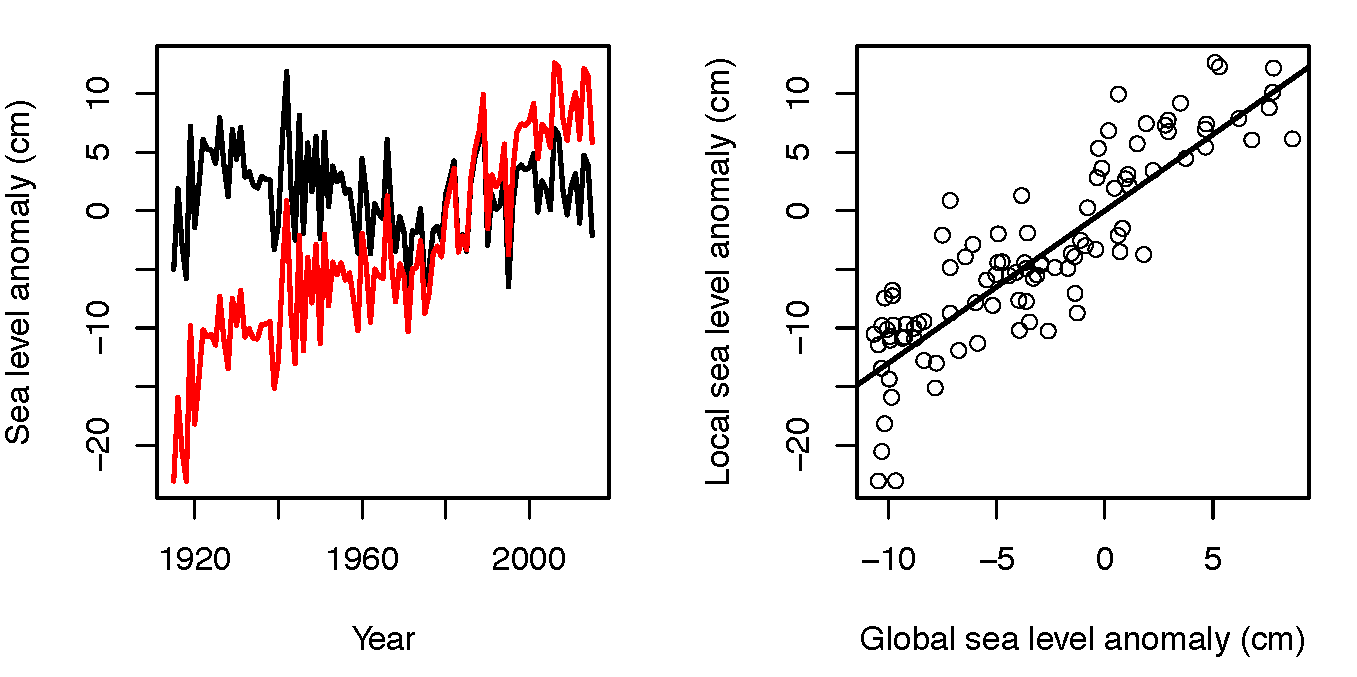
\includegraphics[width=0.75\linewidth]{bergenfit_edit.png}
%DIFDELCMD < %%%
\DIFdelendFL \DIFaddbeginFL 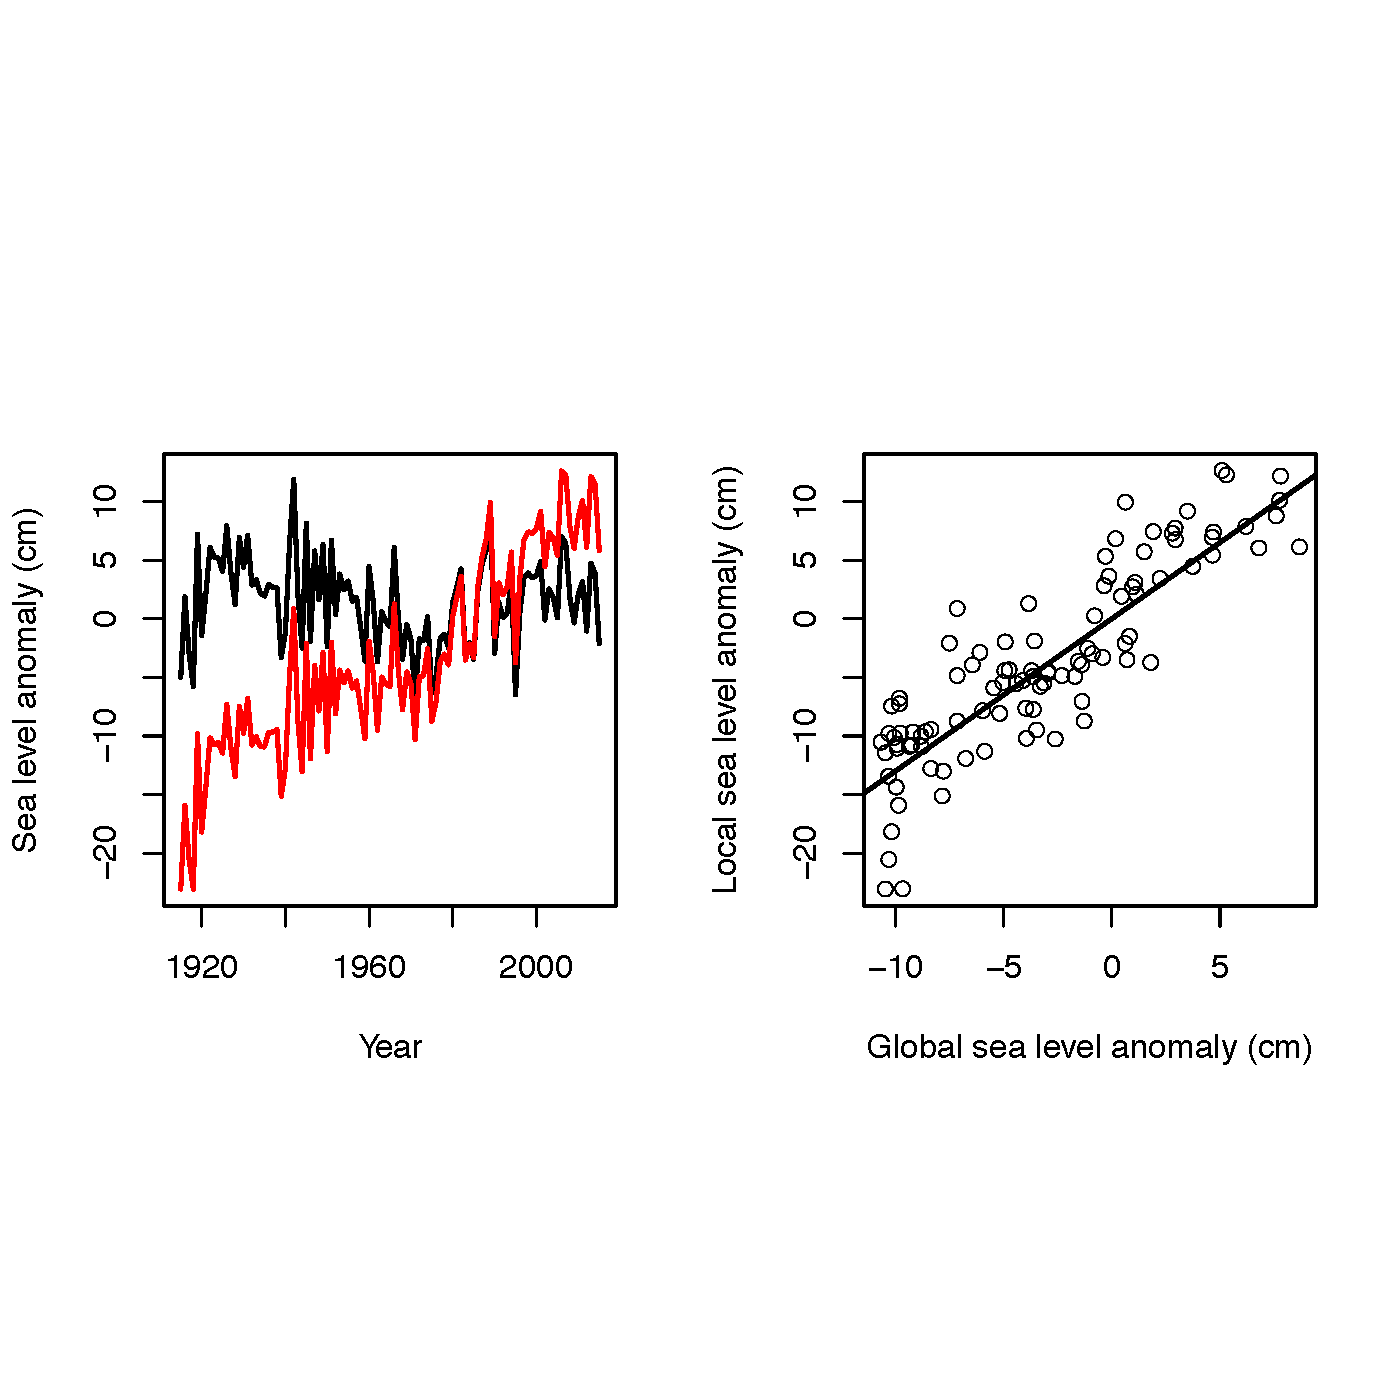
\includegraphics[width=\linewidth]{bergenfit.png}
\DIFaddendFL \caption{ The left figure shows raw (black)and gia-corrected (red) sea level data from Bergen, The right figure relates the gia-corrected Bergen sea level to the global sea level series of \citet{csiro}. The straight line is the time series regression line.}
\label{fig:bergenobs}
\end{center}
\end{figure}

For the relationship between global annual mean temperature and global annual mean sea level rise we use the results from \citet{Bolin2014a}. The left panel of figure \ref{fig:ci} shows the simultaneous 90 \% confidence region for Bergen sea level rise relative to 1999 under scenario RCP 8.5, which is the scenario Norwegian authorities recommend for planning purposes.
\begin{figure}[!hbpt]
\begin{center}
\begin{minipage}{.5\textwidth}

 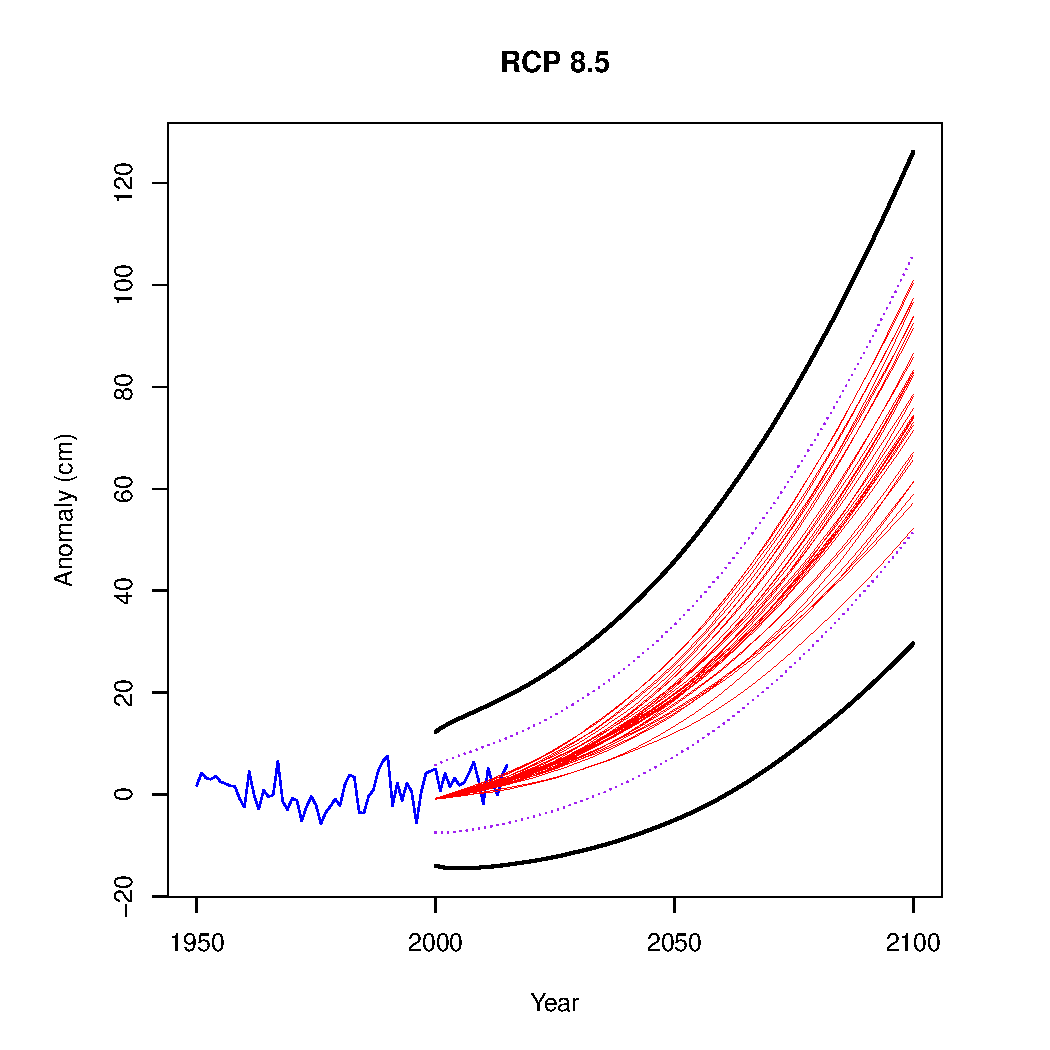
\includegraphics[width=\linewidth]{bergen_ci.pdf}
 % \label{fig:bergenci}

\end{minipage}%
\begin{minipage}{.5\textwidth}

    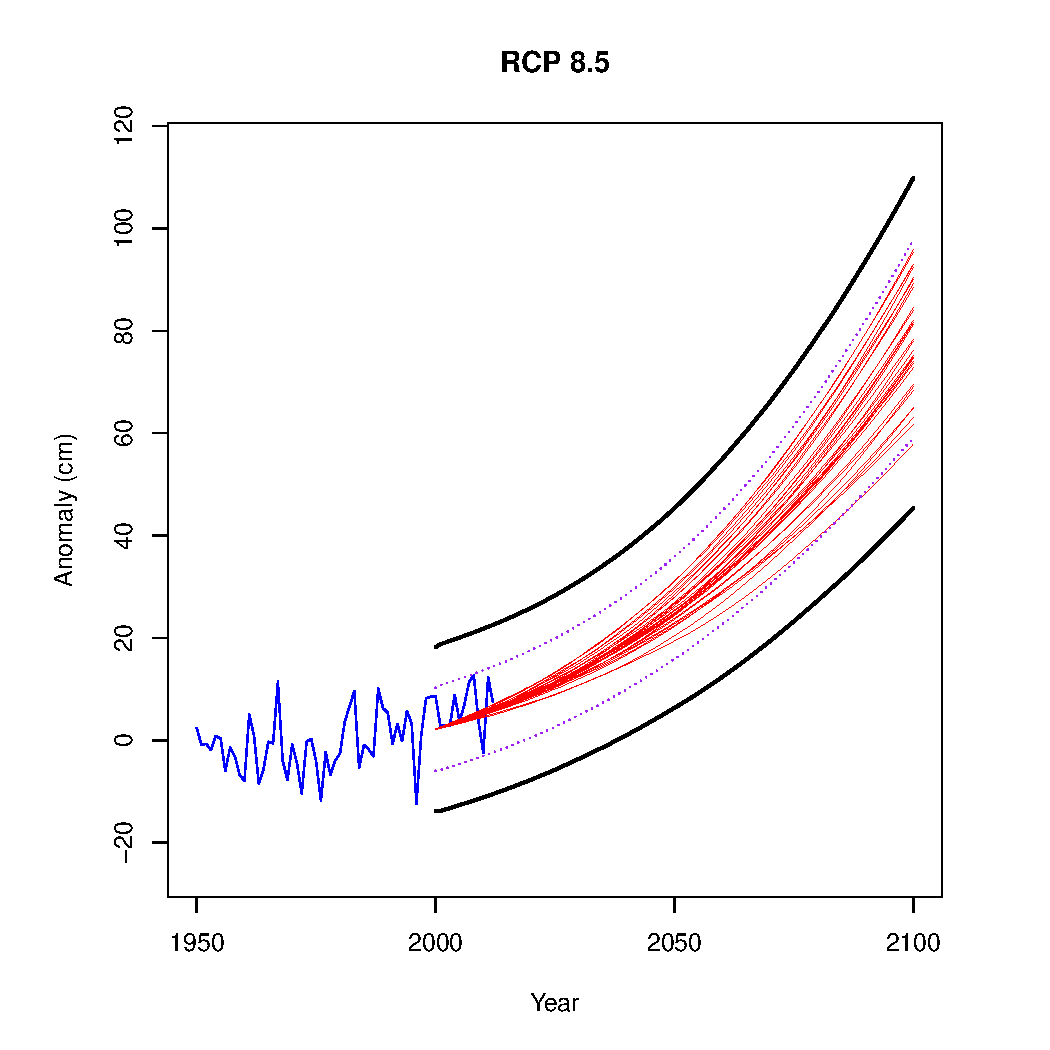
\includegraphics[width=\linewidth]{esbjerg_ci.pdf}
 % \label{fig:esbjergci}

\end{minipage}
\caption{Simultaneous 90\% confidence set (thick black lines) for Bergen (left) and Esbjerg( right) sea level projections for the years 2000-2100 using RCP8.5. The sea level data are shown in blue and end in 2015. The thin red lines are the projections without uncertainty based on each of the climate models. The dashed purple lines connect pointwise confidence intervals for each year. }
\label{fig:ci}
\end{center}
\end{figure}

For Esbjerg, the glacial isostatic adjustment is 0.06 (0.03) cm/yr. The time series regression model relating gia-corrected local to global sea level is an MA(1) model with parameter 0.17 (0.09). The regression slope is 1.02 (0.06). The right panel of figure \ref{fig:ci} shows the simultaneous 90\% confidence region for sea level rise relative to 1999 under scenario RCP 8.5.


\subsection{Timing of adaptation measures \DIFdelbegin \DIFdel{in Bergen}\DIFdelend \DIFaddbegin {\color{blue} \DIFadd{(KdB, TT)}}\DIFaddend }

\DIFdelbegin %DIFDELCMD < \begin{figure}[!hbpt]
%DIFDELCMD < \begin{center}
%DIFDELCMD < 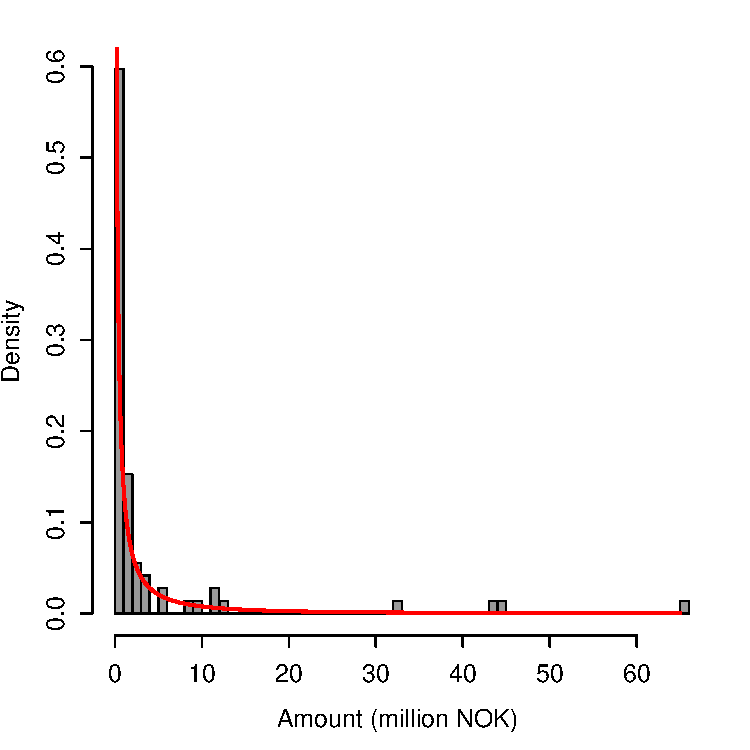
\includegraphics[width=0.5\linewidth]{DecisionAnalysisBergenPartI.pdf}
%DIFDELCMD < %%%
%DIFDELCMD < \caption{%
{%DIFAUXCMD
\DIFdelFL{Estimated distribution of annual damage costs in Bergen for 2015 (red) based on observed annual damage in Hordaland and Rogaland counties 1980-2015 (gray bars).}}
%DIFAUXCMD
%DIFDELCMD < %DIFDELCMD < \label{fig:BergenDamageDist}%%%
%DIFDELCMD < \end{center}
%DIFDELCMD < \end{figure}
%DIFDELCMD < 

%DIFDELCMD < %%%
\DIFdel{Figure~\ref{fig:BergenDamageDist} shows the histogram of observed annual damage costs for Bergen and the associated Burr distribution }\DIFdelend \DIFaddbegin \DIFadd{The histogram of the observed annual damages and the estimated distribution are given in Figure~\ref{fig:BergenDamageDist}}\DIFaddend . The parameter estimates \DIFaddbegin \DIFadd{for the Burr distribution }\DIFaddend are $\hat{\alpha} = 1.27$, $\hat{\gamma} = 0.51$ and $\hat{\theta} = 0.002$. 
\DIFdelbegin \DIFdel{\mbox{%DIFAUXCMD
\citet{bergenreport} }%DIFAUXCMD
discuss several different adaptation options for Bergen. In Figure~\ref{fig:TotalDamageBergen} we consider the optimal timing of an adaptation option that includes two inner barriers at V}%DIFDELCMD < {%%%
\DIFdel{\aa}%DIFDELCMD < }%%%
\DIFdel{gen and Damg}%DIFDELCMD < {%%%
\DIFdel{\aa}%DIFDELCMD < }%%%
\DIFdel{rdssundet, that is, one on each side of central Bergen. The combined construction cost of the two barriers for a protection against 75 cm }\DIFdelend \DIFaddbegin 

\begin{figure}
\begin{center}
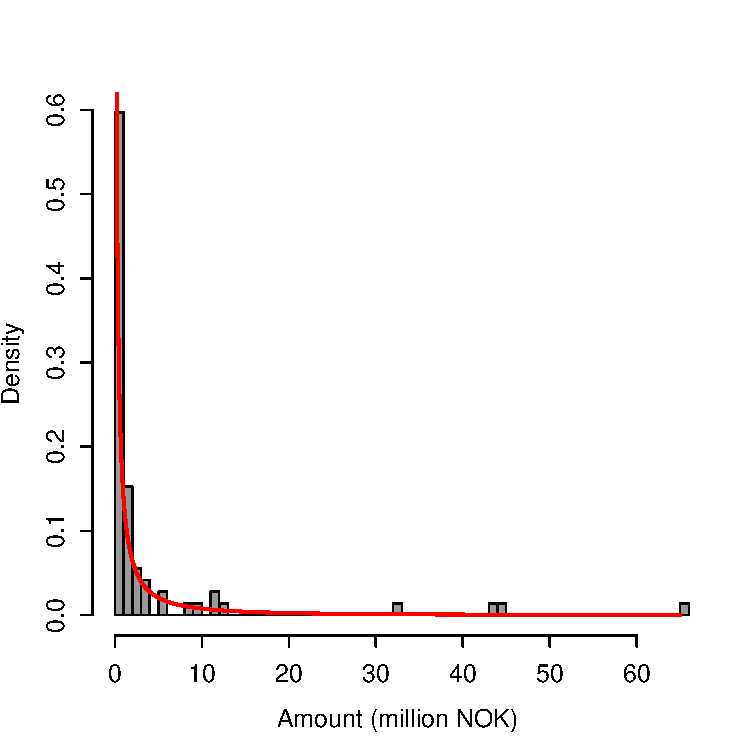
\includegraphics[width=0.5\linewidth]{DamageDistribution.pdf}
\caption{ \DIFaddFL{The estimated distribution of annual storm surge damage in Bergen for 2015 (red) based on observed annual damage in Hordaland and Rogaland 1980-2015 (gray bars). }}
\label{fig:BergenDamageDist}
\end{center}
\end{figure}


\DIFadd{For modelling the relationship between the change in damage and change in sea level we use the results of \mbox{%DIFAUXCMD
\cite{Hallegatte&2013} }%DIFAUXCMD
for 15 European cites: Amsterdam, Athens, Barcelona, Dublin, Glasgow, Hamburg, Helsinki, Copenhagen, Lisbon, London, Marseille, Naples, Porto, Rotterdam and Stockholm. \mbox{%DIFAUXCMD
\cite{Hallegatte&2013} }%DIFAUXCMD
estimate the mean annual flood damage in these cities in 2050 under no sea level change, 20 cm increase and 40 cm increase in sea level. We standardize their results for each city and consider the relative change for 20 and 40 cm increase. We then perform a linear extrapolation to obtain estimated relative changes in damage for a large interval of changes in }\DIFaddend sea level rise\DIFdelbegin \DIFdel{is estimated at 1.13 billion NOK (2015 level)}\DIFdelend \DIFaddbegin \DIFadd{, see Figure~\ref{fig:ChangeInDamage}. Finally, the function $g$ is obtained by sampling from this ensemble of functions with all 15 ensemble members considered equally probable}\DIFaddend . 

\begin{figure}[!hbpt]
\begin{center}
\DIFdelbeginFL %DIFDELCMD < 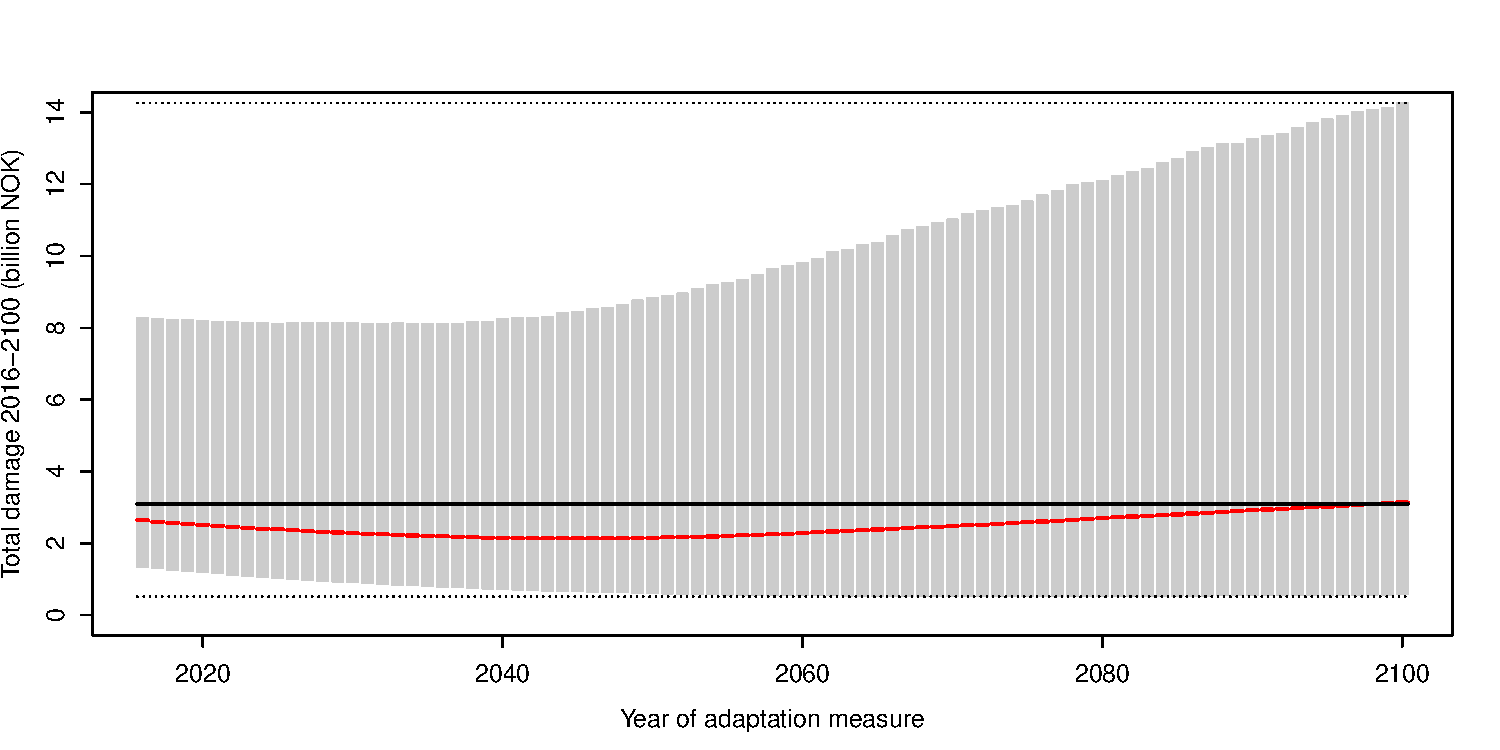
\includegraphics[width=\linewidth]{TotalDamageCostsAdaptation.pdf}
%DIFDELCMD < %%%
\DIFdelendFL \DIFaddbeginFL 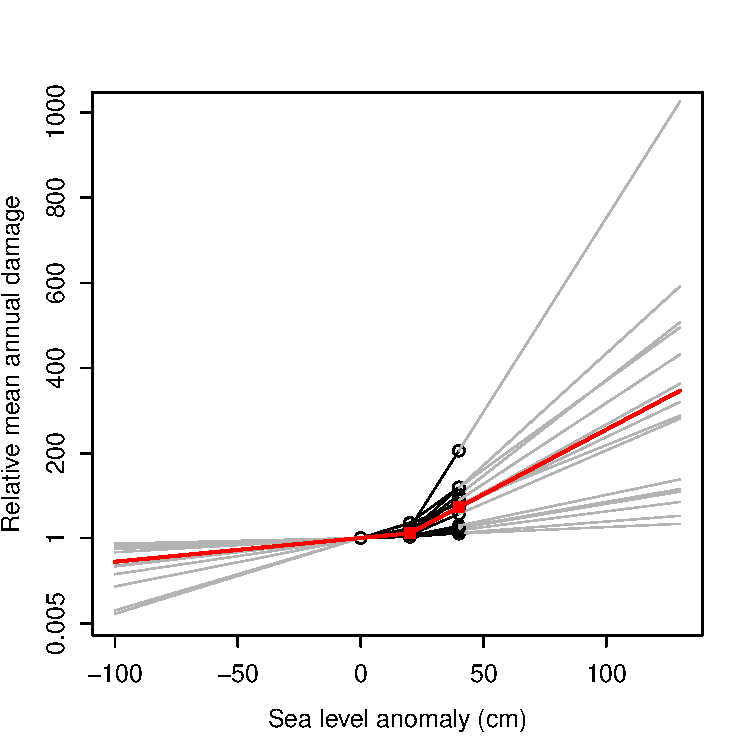
\includegraphics[width=0.5\linewidth]{EuropeanIncreaseLossExtrapolationUncertainty.pdf}
\DIFaddendFL \caption{\DIFdelbeginFL \DIFdelFL{Projected total damage costs }\DIFdelendFL  \DIFaddbeginFL \DIFaddFL{Relative change }\DIFaddendFL in \DIFdelbeginFL \DIFdelFL{Bergen for the time period 2016-2100 }\DIFdelendFL \DIFaddbeginFL \DIFaddFL{mean annual damage }\DIFaddendFL as a function of \DIFdelbeginFL \DIFdelFL{the timing of an adaptation measure consisting of the construction of two inner barriers. The median projection under each adaptation scenario is indicated in red }\DIFdelendFL \DIFaddbeginFL \DIFaddFL{sea level rise for 15 European cites as estimated by \mbox{%DIFAUXCMD
\cite{Hallegatte&2013} }%DIFAUXCMD
(black circles) }\DIFaddendFL with \DIFaddbeginFL \DIFaddFL{linearly extrapolated values indicated by }\DIFaddendFL gray \DIFdelbeginFL \DIFdelFL{bars denoting the 90\% projection intervals}\DIFdelendFL \DIFaddbeginFL \DIFaddFL{lines}\DIFaddendFL . The median \DIFdelbeginFL \DIFdelFL{projected total damage cost under no action is shown with a black line with }\DIFdelendFL \DIFaddbeginFL \DIFaddFL{change and }\DIFaddendFL the corresponding \DIFdelbeginFL \DIFdelFL{90\% projection interval }\DIFdelendFL \DIFaddbeginFL \DIFaddFL{extrapolation are }\DIFaddendFL indicated \DIFdelbeginFL \DIFdelFL{by dotted lines}\DIFdelendFL \DIFaddbeginFL \DIFaddFL{in red}\DIFaddendFL .}
\DIFdelbeginFL %DIFDELCMD < %DIFDELCMD < \label{fig:TotalDamageBergen}%%%
%DIFDELCMD < %%%
\DIFdelendFL \DIFaddbeginFL \label{fig:ChangeInDamage}
\DIFaddendFL \end{center}
\end{figure}


\begin{figure}[!hbpt]
\begin{center}
\DIFdelbeginFL %DIFDELCMD < 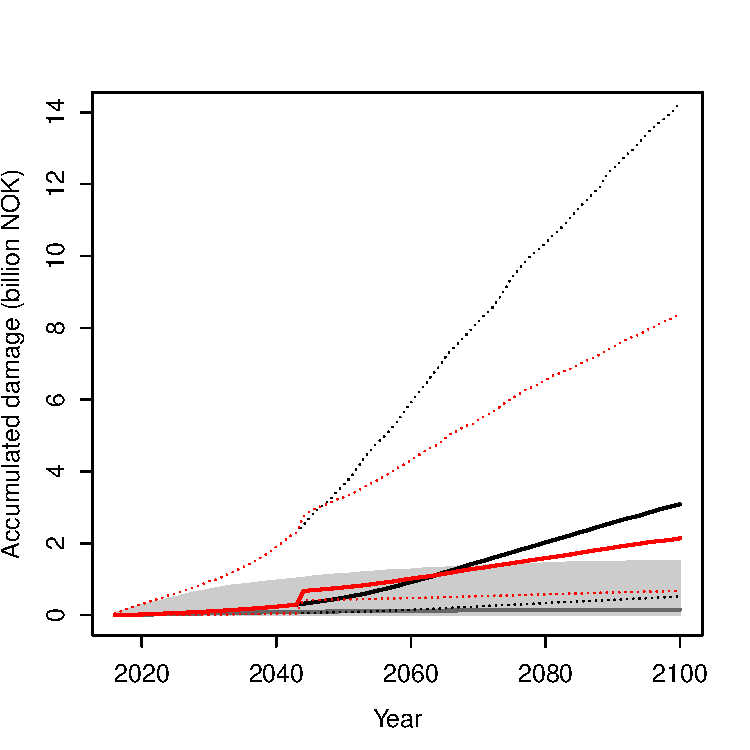
\includegraphics[width=0.5\linewidth]{CumDamageCostsBergen.pdf}
%DIFDELCMD < %%%
\DIFdelendFL \DIFaddbeginFL 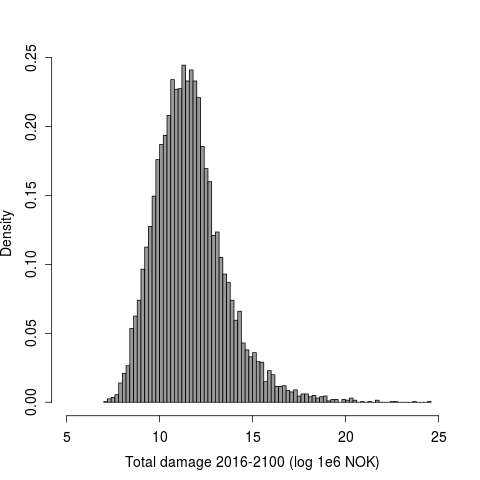
\includegraphics[width=0.5\linewidth]{AccumulatedFutureLoss.png}
\DIFaddendFL \caption{\DIFdelbeginFL \DIFdelFL{Median projected cumulative damage costs in Bergen }\DIFdelendFL \DIFaddbeginFL \DIFaddFL{Distribution of log  accumulated future loss 2016-2100 }\DIFaddendFL under \DIFdelbeginFL \DIFdelFL{constant sea level (gray line), under sea level rise according to }\DIFdelendFL RCP 8.5 \DIFdelbeginFL \DIFdelFL{with }\DIFdelendFL \DIFaddbeginFL \DIFaddFL{and assuming that }\DIFaddendFL no adaptation \DIFdelbeginFL \DIFdelFL{action (black line) and with the construction of two inner barriers in 2047 (red line)}\DIFdelendFL \DIFaddbeginFL \DIFaddFL{measures are implemented}\DIFaddendFL .\DIFdelbeginFL \DIFdelFL{The shaded gray area denotes the 90\% projection interval under constant sea level. Dotted lines indicate the 90\% projection intervals with sea level rise according to RCP 8.5. }\DIFdelendFL } 
\label{fig:NoAction}
\end{center}
\end{figure}


\subsection{\DIFdelbegin \DIFdel{Selection of adaptation measures(?) }\DIFdelend \DIFaddbegin \DIFadd{Identifying flood-prone areas }\DIFaddend {\color{blue} (MD)}}

\DIFdelbegin \DIFdel{A case study focusing on Denmark}\DIFdelend \DIFaddbegin \DIFadd{In 2014 the municipality of Esbjerg adopted its climate adaptation plan }{\color{blue}\DIFadd{(ref)}}\DIFadd{, which will cover the period from 2014-2026, and which aims to reduce the risk of flooding caused by storm surges, heavy rainfall and rising ground water levels, respectively. In the following and based on interviews with end-users from the municipality we will focus on the harbour of Esbjerg and the nearby coastal areas, and we will only consider the hazard of coastal flooding, though evidently in some areas the flood risk is compounded}\DIFaddend . 

\DIFaddbegin \DIFadd{The initial scoping of the climate adaptation plan in Esbjerg was completed in 2014 and includes a preliminary value and risk mapping, considering critical infrastructure and buildings of high cultural and societal value as identified by the municipality, while informed by spatial floods maps for different scenarios corresponding to each of the three different kinds of hydrological events (sea level rise/storm surges, pluvial flooding and rising ground water levels). In terms of coastal floods the mapping considers only one type of storm surge, corresponding to a 20-year return event (based on historical storm surge statistics), and increased sea level due to climate change was not accounted for. 
}

\DIFadd{The risk for any given map area as the probability of, e.g. a certain flood depth, is derived from a hydrological flood model (not including urban drainage system) times a valuation of the consequences, which - similar to the Bergen case - is essentially a loss function associating the flood depth with a measure of economic cost. 
}

\DIFaddend \section{The value of including uncertainty}
\label{unc}

In many cases sea level rise projections are given as a single number for each scenario, usually the mean or median of the ensemble of projections from different climate models (e.g. \citet{climateimpactgroup}). Sometimes the spread of the ensemble is used to assess the uncertainty in the projections (e.g., the Norwegian Environmental Agency recommends using the upper ensemble value for RCP 8.5 as the basis for planning decision, pers. comm. from Even Nilsson, Norwegian Mapping Authority). In our \DIFdelbegin \DIFdel{analysis }\DIFdelend \DIFaddbegin \DIFadd{analysiis }\DIFaddend there are two more sources of uncertainty, namely the two regression models. Figure \ref{fig:unc} shows the single number (vertical black line), the ensemble spread (histogram), the uncertainty including only the global model (red) and the full uncertainty (blue) for Bergen projections of sea level rise relative to 1999 under RCP 8.5. We see that the ensemble range is about 16 cm, whereas the overall uncertainty range is about 40 cm.


\begin{figure}[!hbpt]
\begin{center}
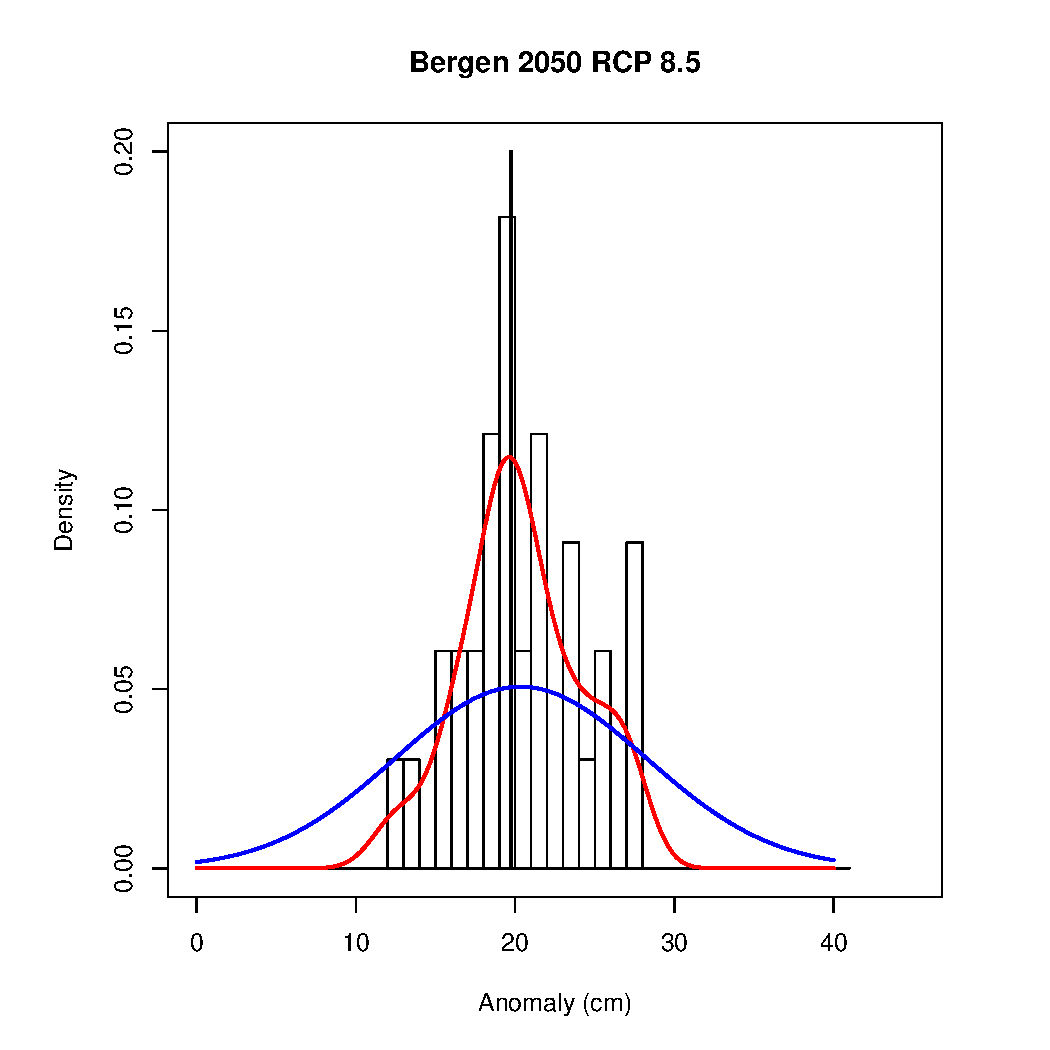
\includegraphics[width=0.5\linewidth]{unc.pdf}
\caption{2050 Bergen sea level projections with uncertainty due to different sources for RCP 8.5. The black vertical line is the median projection (with no uncertainty), while the \DIFdelbeginFL \DIFdelFL{gray }\DIFdelendFL \DIFaddbeginFL \DIFaddFL{grey }\DIFaddendFL histogram corresponds to the spread of the climate models, the red curve adds the uncertainty due to the relation between global temperature and global sea level, and the blue line that due to downscaling global sea level to Bergen. } 
\label{fig:unc}
\end{center}
\end{figure}





%  ACKNOWLEDGMENTS
\begin{acknowledgments}
This work was funded by NordForsk through project number 74456 ``Statistical Analysis of Climate Projections'' (eSACP) and The Research Council of Norway through project number 243953 ``Physical and Statistical Analysis of Climate Extremes in Large Datasets'' (ClimateXL). The source code for the analysis is implemented in the statistical programming language {\tt R} (\DIFdelbegin \DIFdel{\mbox{%DIFAUXCMD
\citet{R}}%DIFAUXCMD
}\DIFdelend \DIFaddbegin \url{http://www.R-project.org}\DIFaddend ) and is available on GitHub at \DIFdelbegin %DIFDELCMD < \url{http://github.com/eSACP/SeaLevelDecisions/Code}%%%
\DIFdelend \DIFaddbegin \url{http://github.com/eSACP/SeaLevelDecisions}\DIFaddend .
\end{acknowledgments}

%%  REFERENCE LIST AND TEXT CITATIONS
% 5\bibliographystyle{../BibTeX/agufull08}

\bibliography{ref.bib}
% Please use ONLY \citet and \citep for reference citations.

%\begin{thebibliography}{37}
%%   Before submitting: copy all the contents into the .bbl LaTeX file here
%%   and run latex again
%\providecommand{\natexlab}[1]{#1}
%\expandafter\ifx\csname urlstyle\endcsname\relax
%  \providecommand{\doi}[1]{doi:\discretionary{}{}{}#1}\else
%  \providecommand{\doi}{doi:\discretionary{}{}{}\begingroup
%  \urlstyle{rm}\Url}\fi


%\end{thebibliography}


%% Enter Figures and Tables here:

\end{document}
